\chapter{Implementing a fast unbounded quantum fanout gate using power-law interactions}
\label{ch:qfo}
In the circuit model for quantum computation, the depth of a quantum circuit is given by the number of layers of non-overlapping quantum gates it contains.
In typical quantum systems, coherence times are a limitation, so low-depth circuits prioritized for the regime of noisy intermediate-scale quantum computers are more desirable \cite{Preskill2018}.
Various proposed models of quantum computation are equivalent up to polynomial overhead, making the definition of the complexity class $\BQP$ insensitive to the model of computation \cite{Bernstein1993,Raussendorf2001,Raussendorf2003,Hoyer2005}.

However, these models can differ in the precise complexity of operations.
As a drastic example, suppose we are given access to a fast unbounded fanout gate
represented by the map
$\ket{x} \ket{y_1} \ket{y_2} \dots$\,$\mapsto$\,$\ket{x}\ket{y_1 \oplus x} \ket{y_2 \oplus x} \cdots$
where the $\oplus$ operator denotes bitwise XOR (bit $y_i$ is flipped if $x$\,$=$\,$1$ and not flipped otherwise). This operation is a reversible analog of a gate that copies $x$ to registers $y_1, y_2, \dots$.
By ``unbounded,'' we mean that there is no limit on the number of bits that can be targeted by this operation.

The unbounded fanout gate makes it possible for constant-depth circuits to perform a number of fundamental quantum arithmetic operations \cite{Hoyer2005}.
Furthermore, unbounded fanout can also reduce the quantum Fourier transform (QFT)---a subroutine of a large class of quantum algorithms, including most famously Shor’s algorithm for integer factorization \cite{Shor1997}---to constant depth as well.
In fact, it enables implementing the entirety of Shor's algorithm by constant-depth circuits with access to a polynomial amount of classical pre- and post-processing \footnote{While the rate-limiting step for factoring is actually modular exponentiation, it is possible to implement this subroutine in logarithmic quantum depth with a polynomial number of classical gates as a pre-computation step, using a standard universal gate set for quantum computing \cite{Cleve2000}. Using the unbounded fanout gate, the quantum circuit for modular exponentiation can be reduced to constant depth as well \cite{Hoyer2005}.}.

While the unbounded fanout gate is clearly a powerful resource for quantum computation, its efficient implementation in physically realizable architectures has not been studied in great depth.
In the standard circuit model---where one may apply single-qubit and two-qubit gates from a standard gate set on arbitrary non-overlapping subsets of the qubits---a fanout gate on $n$ qubits can be implemented optimally in $\Th{\log{n}}$-depth \cite{bigO,Broadbent2009a}.
One may also consider the Hamiltonian model, in which one may apply single-qubit and two-qubit Hamiltonian terms.
In particular, in the Hamiltonian model with all-to-all unit-strength interactions, one can implement the fanout gate in constant time \cite{Fenner2003,Fenner2004}.
However, the assumption of being able to directly apply interactions between two arbitrarily distant qubits does not hold in practice for large quantum computing architectures \cite{Monroe2014,Linke2017,Bapat2018,Childs2019c}.
Mapping these circuits to restricted architectures inevitably leads to overheads and potentially even different asymptotic scaling.
In $d$-dimensional nearest-neighbor architectures, for example, the unbounded fanout gate can only be implemented unitarily in depth $\Th{n^{1/d}}$ \cite{Rosenbaum2013}.
And while there exist protocols that can implement the fanout gate in constant depth on these architectures \cite{Pham2013}, these proposals require intermediate measurements along with classical control---a resource that may be inaccessible in certain near-term experimental systems \cite{Arute2019}.
The overheads resulting from such physical restrictions could therefore limit the potential asymptotic speed-up from a fast quantum fanout.

Systems with power-law interactions, however, present an opportunity for realizing these speed-ups.
Specifically, for a lattice of qubits in $d$ dimensions, the interaction strengths between pairs of qubits separated by a distance $r$ are weighted by a power-law decaying function $1/r^\alpha$.
These long-range interactions are native to many experimental quantum systems and have attracted interest as potential resources for faster quantum information processing. Examples of long-range interactions include dipole-dipole and van der Waals interactions between Rydberg atoms~\cite{Saffman2010,Weimer2012}, and dipole-dipole interactions between polar molecules~\cite{Yan2013} and between defect centers in diamond~\cite{Yao2012,Weimer2012}.
Previous works have explored the acceleration of quantum information processing using strong and tunable power-law interactions between Rydberg states~\cite{Isenhower2011,Molmer2011,Petrosyan2017,Gulliksen2015,Muller2009,Young2020,Levine2019}, which can implement $k$-local gates that control or target simultaneously $k \gg 10$ qubits.
Those gates still have a finite spatial range and can therefore only give a constant-factor speed-up over nearest-neighbor architectures.
Recently, Refs.~\cite{Eldredge2017,Guo2020,Tran2020hierarchylinearlightcones,kuwaharaStrictlyLinearLight2020} gave protocols that take advantage of power-law interactions to quickly transfer a quantum state across a lattice.
As we will show, it is also possible to leverage the power of these interactions to implement quantum gates asymptotically faster than is possible with finite-range interactions \footnote{We note that in Refs.~\cite{Maslov2018,Lu2019}, it was shown that the unbounded quantum fanout could be implemented in trapped-ion systems using a global Molmer-Sorensen gate.
    However, those methods lead to gate durations that scale superlinearly in the system size in order to achieve a certain value of state fidelity and, as such, do not yield an asymptotic speed-up.}.

In this Letter, we propose a protocol for implementing the unbounded fanout gate quickly using engineered Hamiltonians with power-law interactions.
As an application of this protocol, we show that simulating long-range systems with $\al$\,$\le$\,$2d$ for polylogarithmic time or longer is classically intractable, if factoring is classically hard.
As a complement to our upper bounds on the fanout time, we also develop a technique that allows us to prove the tightest-known lower bounds for the time required to implement the QFT and unbounded fanout in a general lattice architecture.

\section{Protocol for fast fanout using long-range interactions}
To perform a fanout gate on $n$ logical qubits, we
employ as subroutines modified versions of the state transfer protocols from Refs.~\cite{Eldredge2017} and \cite{Tran2021a} to generate a many-body entangled state in $\O{\polylog(n)}$ time using long-range interactions with $\al$\,$<$\,$2d$.

As an intermediate step, both state-transfer protocols ``broadcast'' a single-qubit state into the corresponding Greenberger–Horne–Zeilinger (GHZ)-like state:
\begin{equation}
    \label{eq:longrangebroadcast}
	(\psi_0 \ket{0} + \psi_1 \ket{1})\otimes \ket{0 0 \dots 0} \mapsto \psi_0 \ket{0 0  \dots 0} + \psi_1 \ket{1 1 \dots 1},
\end{equation}
where $\psi_0, \psi_1$\,$\in$\,$\mathbb{C}$ and $|\psi_0|^2$\,$+$\,$|\psi_1|^2$\,$=$\,$1$.
In the case of Ref.~\cite{Eldredge2017}, this long-range broadcast is achieved by performing a sequence of cascaded controlled-\textsc{Not} (\textsc{CNot}) gates---similar to the standard gate-based implementation of the unbounded fanout gate.
The \textsc{CNot} gate from qubit $i$ to qubit $j$ can be implemented by a Hamiltonian $H_{ij}$\,$=$\,$h_{ij} \ketbra{1}_i$\,$\otimes$\,$X_j$ acting for time $t$\,$=$\,$\pi/(2h_{ij})$, up to a local unitary.
Applying a Hamiltonian $H(t)$\,$=$\,$\sum_{ij} H_{ij}(t)$, which variously turns on/off interactions between pairs of qubits at different times, allows one to implement the broadcast in \cref{eq:longrangebroadcast}.

By using Hamiltonians with long-range interactions $h_{ij}$ satisfying $\norm{h_{ij}}$\,$\le$\,$1/r_{ij}^\al$, it is possible to implement the broadcast operation asymptotically faster than with short-range interactions---a statement that we will prove rigorously later in the text.
For a system of $n$ qubits, Refs.~\cite{Eldredge2017} and \cite{Tran2021a} showed that this broadcast time depends on the power-law exponent $\al$ and the dimension of the system $d$ as follows:
\begin{equation}
\label{eq:statetransfertimes_new}
	\tghz =
  \begin{cases}
    \O{n^0} & \alpha < d
    \\ \O{\log n} & \alpha = d
    \\ \O{\log^{\kappa_\alpha} n }& \alpha \in (d,2d)
    \\ \O{e^{\gamma\sqrt{\log n}}}& \al = 2d
    \\ \O{n^{\min(\al/d - 2,1)}} & \alpha > 2d,
  \end{cases}
\end{equation}
for constants $\gamma = 3\sqrt{d}$ and $\kappa_\alpha = \log 4/\log(2d/\alpha)$.
We term the broadcast time $t_{\text{GHZ}}$, since it corresponds to the GHZ-state-construction time when $\psi_0$\,$=$\,$\psi_1$\,$=1/\sqrt{2}$.
This long-range broadcast is not the same as fanout because it requires that all intermediary qubits (besides the first qubit) be initialized in the $\ket{0}$ state.
However, as we now show, it is possible to adapt the broadcast protocol to implement the fanout gate in time $\tghz$ using $n$ ancillary qubits.

\begin{figure}[t]
\centering
    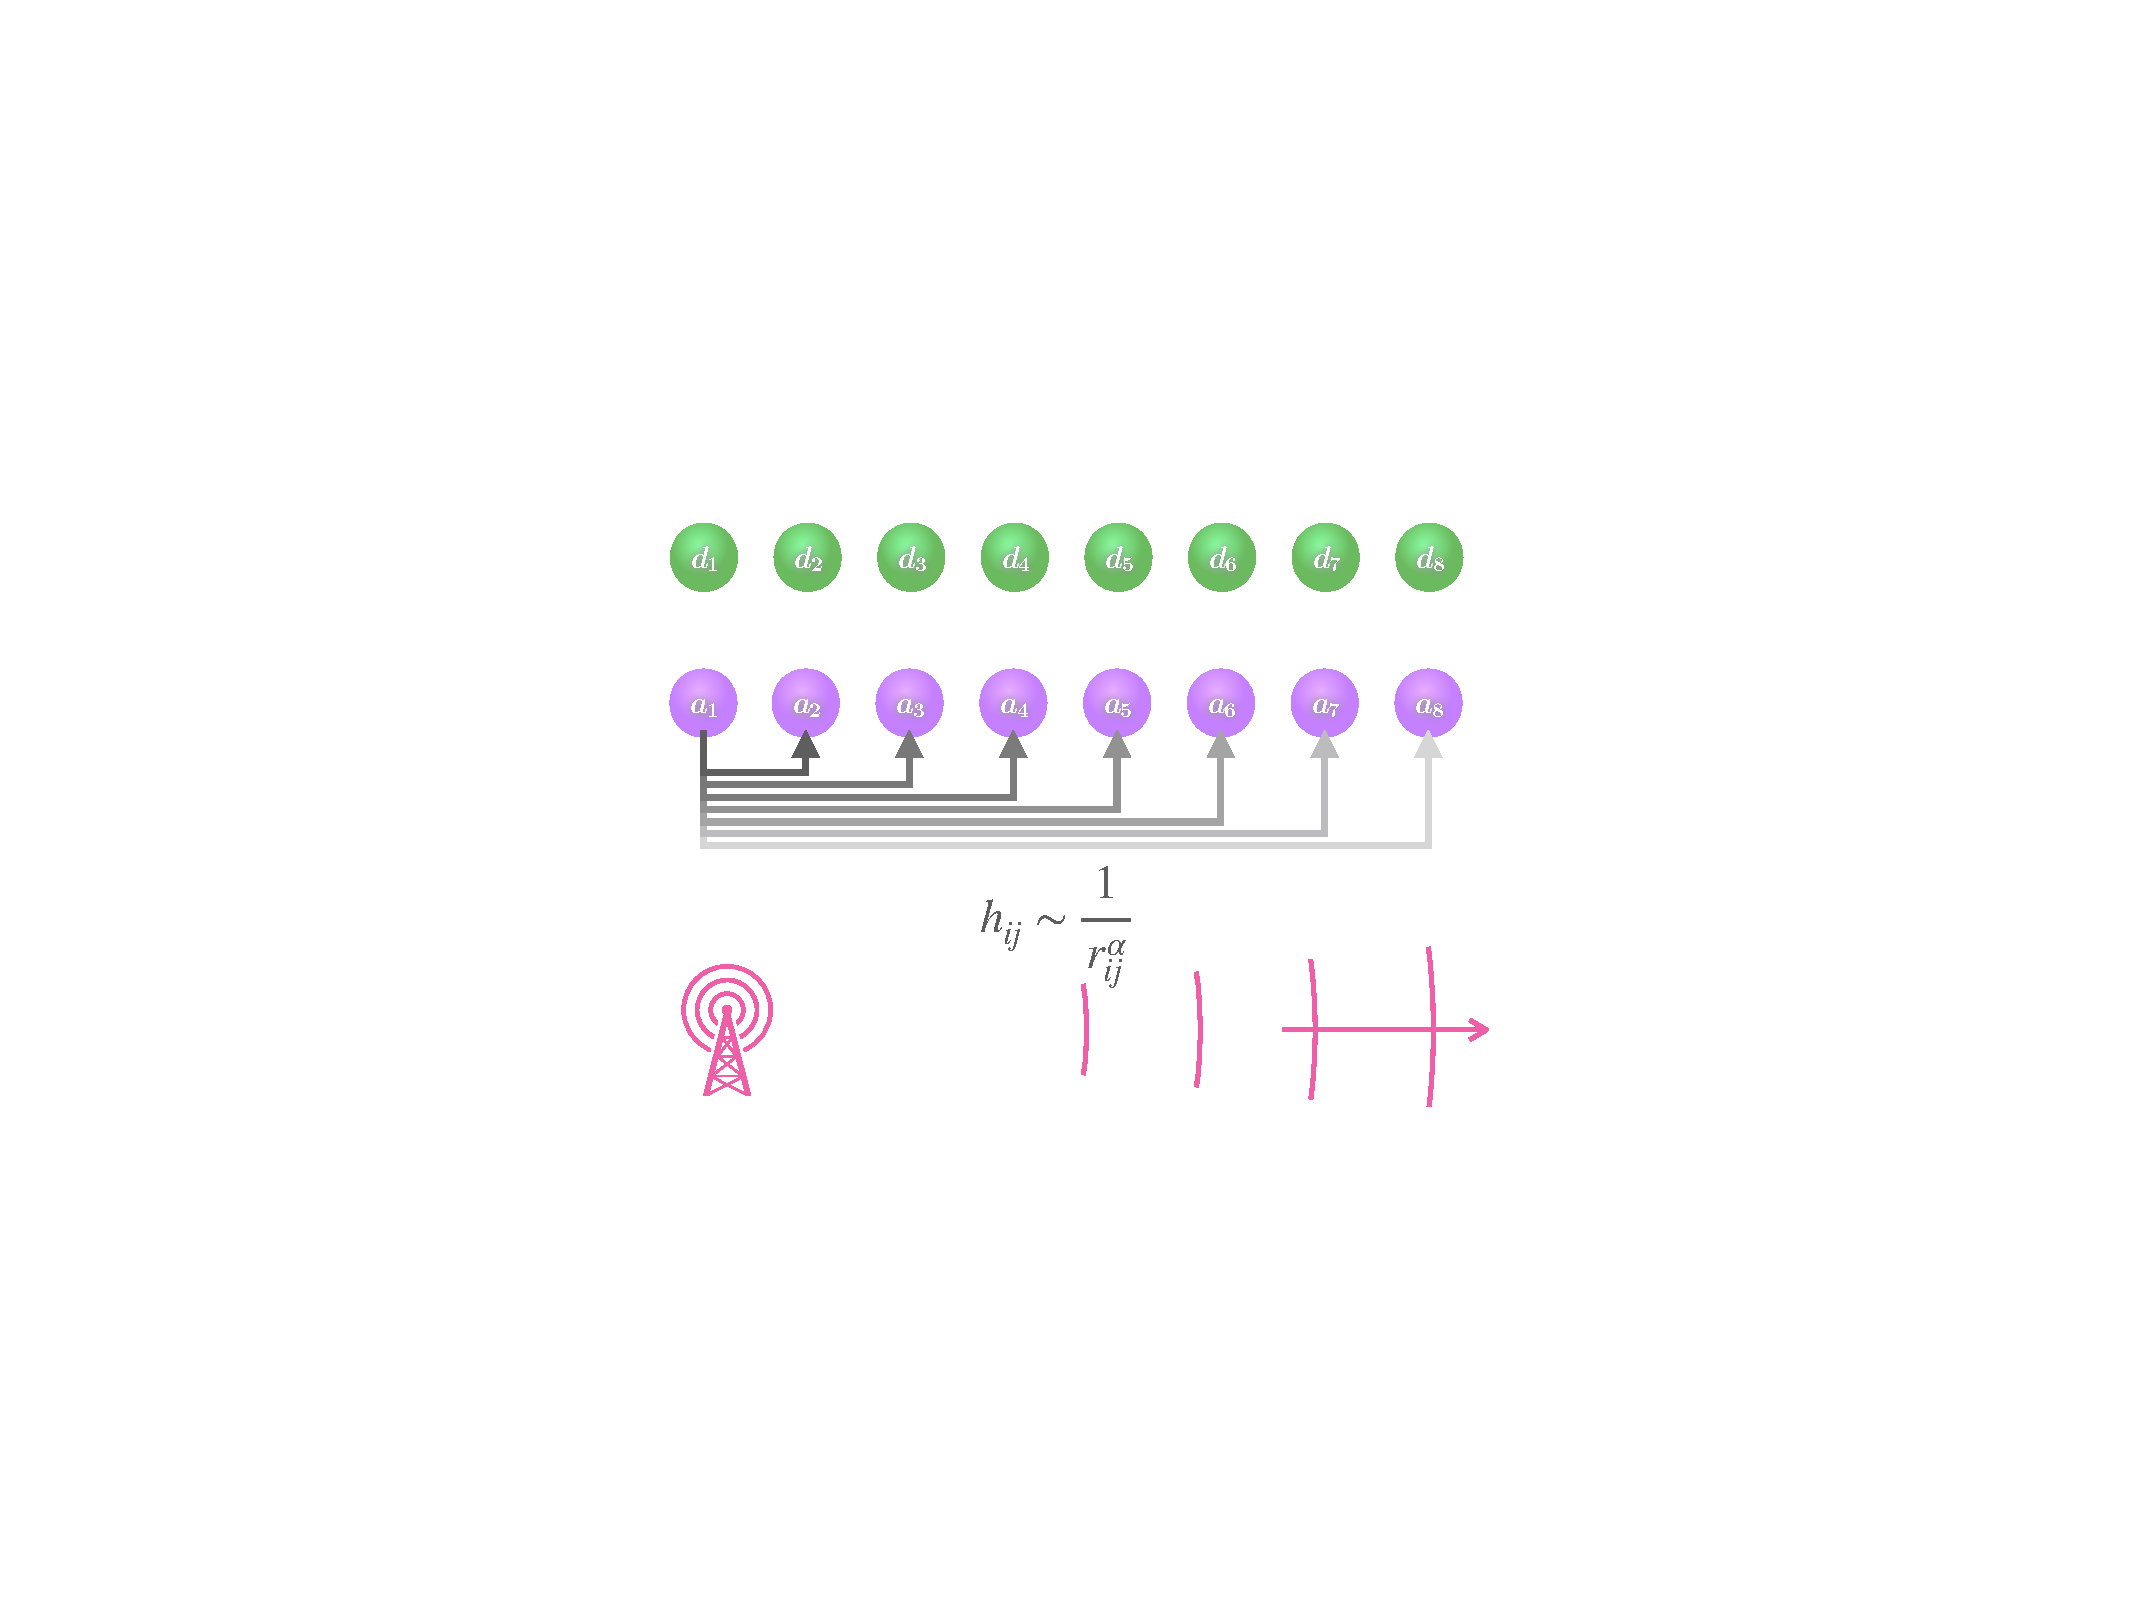
\includegraphics[scale=0.45]{figures/fanoutgate.pdf}
\centering
  \caption{A protocol for a fast unbounded quantum fanout gate using long-range interactions, depicted here for a 1D lattice.
  The layout consists of a chain of data qubits, along with their adjacent ancillary qubits that are initialized to $\ket{0}$.
  (a) The first step is a local controlled-\textsc{Not} (\textsc{CNot}) gate from $\ket{d_1}$ to $\ket{a_1}$.
  (b) The application of the long-range ``broadcast'' from $\ket{a_1}$ to the rest of the ancillary qubits $\ket{a_i}$ creates a GHZ-like state in Eq.\,(\ref{eq:longrangebroadcast}) for the ancillary qubits together with the first data qubit.
  (c) We apply \textsc{CNot} gates from ancillary qubit $\ket{a_i}$ to the data qubit $\ket{d_i}$, which can be done in parallel. After this step, we reverse process (b) and process (a) to return the ancillary qubits to $\ket{0}$ (not redrawn here). }
  \label{fig:broadcast}
\end{figure}

Consider a system of $n$ data qubits arranged on a $d$-dimensional lattice.
Furthermore, assume there are $n$ ancillary qubits, each located adjacent to one of the original qubits.
We denote the qubits as $\ket{d_1}, \ket{d_2}, \dots, \ket{d_n}$ and $\ket{a_1}, \ket{a_2}, \dots, \ket{a_n}$ for data and ancilla, respectively.
Suppose we want to perform fanout with $\ket{d_1}$ as control, and that all ancillae are guaranteed to be in state $\ket{0}$.
Then the sequence of operations in \cref{alg:fastfanout} (also depicted graphically in \cref{fig:broadcast}) implements the fanout operation.

In addition to accomplishing fanout, this protocol returns the ancillary qubits to the $\ket{0}$ state.
Modulo the $\O{n}$ short-range operations that can be done in parallel in a single time step, the protocol requires time $2 t_\mathrm{GHZ}$.
Hence, it can implement the fanout gate in time that is constant for $\alpha$\,$<$\,$d$, polylogarithmic for $d$\,$\le$\,$\alpha$\,$<$\,$2d$, and polynomial for $\alpha$\,$>$\,$2d$.

\begin{algorithm}[H]
% \renewcommand{\thealgorithm}{}
  \caption{Implementing fanout with long-range interactions}
  \label{alg:fastfanout}
  \begin{algorithmic}[1]
   \State Initialize ancillary qubits: $\ket{a_i}$\,$\gets$\,$\ket{0}$ for $i$\,$=$\,$1$ to $n$
  \State \textsc{CNot}($\ket{d_1}$\,$\ra$\,$\ket{a_1}$)
  \Statex $\bigtriangledown$ Apply broadcast operation as shown in \cref{eq:longrangebroadcast} to ancillae:
  \State \textsc{LongRangeBroadcast}($\ket{a_1}$\,$\ra$\,$\ket{a_2},\dots,\ket{a_n}$)
  \Statex $\bigtriangledown$ \textbf{parfor} indicates that \textbf{for}-loop can be implemented in \textbf{par}allel
  \ParFor {$i$\,$=$\,$2$ to $n$}
    \State \textsc{CNot}($\ket{a_i}$\,$\ra$\,$\ket{d_{i}}$)
    \Comment{\parbox[t]{.45\linewidth}{{Transfer} fanout to data qubits}}
  \EndParFor
  \Statex $\bigtriangledown$ Apply broadcast operation in reverse to uncompute ancillae
  \State \textsc{ReverseLongRangeBroadcast}($\ket{a_2},\dots,\ket{a_n}$\,$\ra$\,$\ket{a_1}$)
  \State \textsc{CNot}($\ket{d_1}$\,$\ra$\,$\ket{a_1}$)
  \end{algorithmic}
\end{algorithm}

We briefly comment on the constant-depth implementation of the QFT and Shor's algorithm using the unbounded fanout gate.
An $n$-qubit QFT circuit can be performed with $\O{n\log n}$ gates to $1/\text{poly}(n)$ precision \cite{Coppersmith94}.
Using unbounded fanout, the circuit can be reduced to constant depth with $\O{n\log n}$ ancillary qubits \cite{Hoyer2005}.
We note that including these ancillae in the lattice would not change the asymptotic scaling of our protocol for $\al$\,$<$\,$2d$, since $\tghz$ is $\O{\polylog(n)}$ in this regime.

We also remark on the potential ways of performing the fast fanout gate experimentally.
One method would be to use two different qubit realizations for the data and ancillary qubits,  with the former interfacing with the latter through local interactions.
For example, one may consider a system of fermionic alkaline-earth atoms, with each atom's electron on the clock transition acting as an ancillary qubit, its nuclear spin as the data qubit, and with long-range Rydberg-Rydberg interactions between electrons.
In this heterogeneous case, the $n$ $\textsc{CNot}$ gates between the data and ancilla qubits of our protocol would be straightforward to implement in parallel \cite{Gorshkov2009}.
Alternatively, one may consider implementing the protocol entirely in a system of Rydberg atoms using power-law interactions of different strengths.
This could be done using a gate based on %diagonal
van der Waals interactions ($\al = 6$) to implement the short-range $\textsc{CNot}$ gates between data and ancilla qubits, and then rotating into a new basis in order to implement the long-range broadcast interaction using dipole-dipole interactions ($\al = 3$).
We provide more discussion on the implementation of the protocol in the Supplemental Material \cite{SM}.

\section{Intractability of classical simulation of long-range systems with $\al$\,$<$\,$2d$}
As a corollary, the protocol shows that long-range interacting systems with $\al$\,$<$\,$2d$ evolving for time polylogarithmic in $n$ or longer are difficult to simulate classically in the worst case.
% By this we mean that in order to approximately sample from the time-evolved state to within constant total-variation-distance error $\varepsilon$, a classical computer would require time at least superpolynomial in the system size \cite{note_constanterror}.
The argument operates by a complexity-theoretic reduction from integer factoring, a problem that is assumed to be difficult for classical computers with the ability to use random bits (\textsc{Factoring} $\notin$\,$\BPP$).
This assumption suggests that the simulation of long-range systems could provide an avenue towards a potentially useful experimental demonstration of quantum computational advantage.

The argument proceeds as follows.
The time required to implement the fanout gate using \cref{alg:fastfanout} is $\O{\polylog(n)}$ for $\al$\,$<$\,$2d$.
It is possible to implement Shor's order-finding algorithm in time $\O{t_\mathrm{FO}}$ using a small amount of classical pre-processing (polynomial in $n$) \cite{Cleve2000,Hoyer2005}.
Using the ability to sample from the output of the order-finding algorithm to error $\varepsilon$\,$<$\,$0.4$\,$<$\,$4/\pi^2$, classically efficient post-processing can output a factor of an $n$-bit integer with probability $\W{1}$ \cite{Shor1997}.
Therefore, if it were possible to efficiently sample from the output distribution in long-range systems with $\al$\,$<$\,$2d$ for evolution-time $t$\,$=$\,$\mathcal{O}(\log n)$, then it would be possible to factor $n$-bit integers efficiently as well.
The best classical algorithm currently known for factoring an $n$-bit integer takes runtime $\exp[\mathcal{O}(\sqrt{n \log n})]$ \cite{Lenstra1992} and the problem is widely believed to be classically intractable.
This stands in contrast to systems with finite-range interactions in 1D, for which efficient classical simulation is possible up to any time satisfying $t$\,$\leq$\,$\O{\log n}$ \cite{Osborne2006}.
Under the complexity assumption mentioned above (\textsc{Factoring} $\notin$\,$\BPP$), we have shown that this result is not fully generalizable to long-range interacting systems with $\al$\,$<$\,$2d$\footnote{We note that a similar result could have been achieved using the fact that constant-depth quantum circuits with two fanouts are not classically simulable unless $P = PP$ \cite{Takahashi2014}.}.


%%%%%%Lower bounds on the time required to implement QFT and fanout%%%%%%%

\section{Lower bounds on the time required to implement QFT and fanout}
In previous sections, we found upper bounds to the time required to implement fanout---and by corollary, the QFT.
As a way to benchmark our long-range protocol, we now proceed to discuss lower bounds for implementing fanout and the QFT.
Recall that the protocol in \cref{alg:fastfanout} can implement fanout in time $\tghz$, which scales as $\O{\polylog(n)}$ for long-range systems with $\alpha$\,$<$\,$2d$.
In this section, we show that such fast asymptotic runtimes cannot be achieved in architectures with strict locality constraints.

In Ref.\,\cite{Maslov2007}, Maslov showed that a specific way of implementing the QFT requires $\W n$ depth on the 1D  nearest-neighbor architecture, though this does not rule out other QFT implementations with potentially sublinear depth.
Here, we devise a technique that yields a lower bound of $\W {n^{1/d}}$ for the time required to perform a QFT in the Hamiltonian model.
This result strengthens and generalizes Maslov's bound to higher dimensions and to the Hamiltonian model.
In addition, we show that the same lower bound applies even to circuits that perform the QFT approximately.

Our $\W {n^{1/d}}$ lower bound holds for any lattice system with finite velocities of information spreading, which include short-range interactions (i.e., finite-ranged or exponentially decaying) and power-law interactions with $\al$\,$>$\,$2$ in one dimension or $\alpha$\,$>$\,$2d$\,$+$\,$1$ for $d$\,$>$\,$1$ \cite{Lieb1972,Chen2019,kuwaharaStrictlyLinearLight2020}.
Combined with our results above, this implies that systems with long-range interactions with $\al$\,$<$\,$2d$ can implement the QFT and fanout asymptotically faster than more weakly interacting systems.

The intuitive idea behind our proof is that the QFT unitary can spread out operators in a certain precise sense, a task that can be bounded by the ``Frobenius-norm light cone'' of Ref.\,\cite{Tran2020hierarchylinearlightcones}.
The fact that this light cone imposes a finite speed limit on information propagation in short-range interacting systems implies that the minimum time $t_2(r)$ required for operator-spreading is proportional to the distance between qubits $r$.
This constrains the implementation time for the QFT, denoted $t_\mathrm{QFT}$, by $\W {n^{1/d}}$, from which the circuit-depth lower bound follows.
The same Frobenius-norm bound also constrains the time required to implement the approximate QFT (AQFT).

We consider the $4^n$-dimensional vector space of $n$-qubit operators for which the set of Pauli operators $\{I,X,Y,Z\}^{\otimes n}$ forms a basis.
We quantify operator spreading outside a region of radius $r$ as follows.
Taking an operator $|O)$ initially supported on site 1, we measure the weight of its time-evolved version, $|O(t))$, on sites at distance $r$ (and beyond) using a \emph{projection} operator $\mathcal{Q}_{r}$, which projects onto strings of Pauli operators that act nontrivially on at least one site at distance $r$ or greater.
We measure the weight of this projected operator $|O_r)$\,$\coloneqq$\,$\mathcal{Q}_{r}|O(t))$ via the (squared) normalized Frobenius norm $\norm{O_r}_F^2$\,$\coloneqq$\,$\Tr(O_r^\dag O_r)/2^n$, which coincides with the Euclidean norm over the operator space, $(O_r|O_r)$ \footnote{See Ref.\,\cite{Tran2020a} for a more precise definition.
    We note that our projector $\mathcal{Q}_r$ is a variation on the $\mathbb{Q}_r$ used in {Ref.\,\cite{Tran2020a}}.
    Specifically, for $d=1$, they are related via $\mathcal{Q}_r = \sum_{x:\,|x|\ge r} \mathbb{Q}_x$.}.
We define $t_2(r)$ to be the minimal time after which $\norm{O_r}_F^2$ is able to achieve a predetermined constant value \cite{Tran2020hierarchylinearlightcones}.
% on sites at distance $r$ or beyond. \cite{note_t2r}.

We show that operators spread by the action of the QFT can have high weight on distant regions,
which implies that $t_\mathrm{QFT}$\,$\geq$\,$t_2(r)$.
Recall that the QFT operator on $n$ qubits is defined as $U_\mathrm{QFT} \coloneqq \sum_{y,z=0}^{2^n-1} \ketbra{y}{z} {\omega^{yz}}/{\sqrt{2^n}}$, where $\ket{y}$ $(\ket{z})$ is an $n$-qubit state that encodes the binary representation of $y$ ($z$) and $\omega = e^{2\pi i/2^n}$.
Then the following lemma holds:
\begin{lemma*} \label{lem_qft_weight}
Let $U_\mathrm{QFT}$ be the QFT operator on $n$ qubits arranged in a $d$-dimensional lattice such that the first and $n$-th qubits are located a distance $r$\,$=$\,$\Theta(n^{1/d})$ apart.
Then $U_\mathrm{QFT}^\dag Z_1 U_\mathrm{QFT}$\,$=:$\,$Z_1' $ is an operator with at least constant weight at distance $r$.
\end{lemma*}

We defer the (short) proof of this Lemma to the Supplementary Material \cite{SM}.
As a result of the Lemma, $t_\mathrm{QFT}$ follows the light cone defined by the normalized Frobenius norm, which is at least as stringent as the Lieb-Robinson light cone.
This leads directly to the following theorem:
%
% \begin{proof}
% We explicitly compute the weight of the operator $Z_1'$ on site $n$.
% define $\omega$\,$:=$\,$e^{2\pi i/2^n}$.
% The QFT operation on $n$ qubits is defined as $\sum_{y,z=0}^{2^n-1} \ketbra{y}{z} {\omega^{yz}}/{\sqrt{2^n}}$, where we interpret the bit string $y_1, y_2, \ldots, y_n$ as a binary representation of a number $y$\,$\in$\,$\{0,1,\ldots, 2^n -1\}$ in the canonical ordering, i.e.\ $y$\,$=$\,$y_1 2^{n-1}$\,$+$\,$y_2 2^{n-2}$\,$+$\,$\cdots$\,$+$\,$y_n$.
% The inverse of the QFT is obtained simply by taking $\omega$\,$\rightarrow$\,$\omega^{-1}$.
% First, we compute
% \begin{align}
% Z_1' &= \sum_{x,y,z=0}^{2^n-1} \ketbra{z}{y} \frac{\omega^{-z y}(-1)^{y_1} \omega^{yx}}{2^n} \ketbra{y}{x}.
% \end{align}
% We divide the sum over $y$ into two cases, $y_1$\,$=$\,$0$ and $y_1$\,$=$\,$1$:
% \begin{align}
% Z_1' &= \frac{1}{2^n}\sum_{x,z=0}^{2^n-1} \ketbra{z}{x} \left(\sum_{y:\, y_1 = 0} \omega^{(x-z) y} - \sum_{y:\, y_1= 1} \omega^{(x-z) y}\right).
% \end{align}
% We can compute these sums separately, giving
% \begin{align}
% \label{eq:zoneprime}
% Z_1' = \frac{1}{2^{n-1}}\sum_{x\neq z}\ketbra{z}{x} \frac{1 - (-1)^{(x-z)}}{1-\omega^{x-z}}.
% \end{align}
% The nonzero terms in the sum on the right-hand side of \cref{eq:zoneprime} occur when $x-z$ is odd, i.e., when $x_n$\,$-$\,$z_n$\,$=$\,$1 \bmod 2$.
% Therefore, the only terms that remain are off-diagonal on qubit $n$ or, equivalently, contain only the $X_n$ or $Y_n$ Pauli operators.
% This implies that $Z_1'$ has all its weight on operators acting nontrivially at distance $r$---formally, that $\mathcal{Q}_r |Z_1')$\,$=$\,$|Z_1')$.
% \end{proof}

%
\begin{theorem*}  \label{thm:QFTlowerbounds}
  For systems with finite-range or exponentially-decaying interactions in $d$ dimensions, the time required to implement the QFT unitary is lower bounded by $t_\mathrm{QFT}$\,$= $\,$\W{r}$, where $r$\,$=$\,$\Theta(n^{1/d})$ is the distance between the first and $n$-th qubits.

  For systems with long-range interactions, the Lieb-Robinson light cone gives the following bounds \cite{kuwaharaStrictlyLinearLight2020,Tran2019a,Hastings2006,Tran2021b}:
  \begin{align}
  \label{eq:LRlowerbounds}
   t_\mathrm{QFT} =
   \begin{cases}
      \W{1}, & \al = d
      \\ \W{\log r}, & \alpha \in (d,2d]
      \\ \W{r^{\alpha-2d}}, & \alpha \in (2d,2d+1]
      \\ \W{r}, & \alpha > 2d + 1.
    \end{cases}
  \end{align}
  The Frobenius light cone gives the following (tighter) bounds \cite{Kuwahara2021,Chen2021Frobenius}:
  \begin{align}
  \label{eq:Froblowerbounds}
   t_\mathrm{QFT} =
   \begin{cases}
      \W{r^{\frac{2\al-2d}{2\alpha-d+1}}}, & \al \in (d,2d]
      \\ \W{r^{\alpha -1}}, & \alpha \in (1,2], d=1
      \\ \W{r}, & \alpha > 2, d=1.
   \end{cases}
  \end{align}
\end{theorem*}
%
We note that the lower bounds in the Theorem also apply to the fanout time, $t_\mathrm{FO}$, through the observation that fanout also performs operator spreading (using $X_1$ instead of $Z_1$).
We emphasize that these bounds pertain to the Hamiltonian model, where commuting terms can be implemented simultaneously and state transfer could in theory be done in $o(1)$ time for sufficiently small $\alpha$.

We observe that the QFT can implement quantum state transfer as well.
The goal of state transfer is to find a unitary $V$ such that
$V \bigl(\ket{\psi} \otimes \ket{0}^{\otimes n-1}\bigr)$\,$=$\,$\ket{0}^{\otimes n-1}$\,$\otimes $\,$\ket{\psi}$ \cite{Eldredge2017,Epstein2017}.
The unitary $V$\,$=$\,$H^{\otimes n} U_\mathrm{QFT}$ (where $H$ represents the single-qubit Hadamard gate) satisfies this definition of state transfer.

For the AQFT, the lower bound follows in a similar fashion.
The circuit that implements the QFT approximately with error $\varepsilon$ can be represented by a unitary $\tilde{U}_\mathrm{QFT}$ such that $\|U_\mathrm{QFT}-\tilde {U}_\mathrm{QFT}\|\leq \varepsilon$ \cite{Cleve2000}.
In the Supplemental Material, we show that the operator $\tilde {U}_\mathrm{QFT}^\dag Z_1 \tilde {U}_\mathrm{QFT}$ also has large support on sites beyond distance $r$ as well, implying that the lower bounds in \cref{eq:LRlowerbounds,eq:Froblowerbounds} also hold for the AQFT.

\section{Conclusions and Outlook}
In
summary, we have developed a fast protocol for the unbounded fanout gate using power-law interactions.
For $\al$\,$\le$\,$2d$, the protocol can perform the gate parametrically faster than is possible with short-range interactions.
In particular, for experimentally realizable dipole-dipole interactions with $\al$\,$=$\,$3$ in two and three dimensions, as well as van der Waals interactions with $\al$\,$=$\,$6$ in three dimensions, the fast fanout protocol allows the quantum Fourier transform and Shor's algorithm to be performed in time that scales subpolynomially in the number of qubits.
As a corollary, we showed that the classical simulation of long-range systems with $\al$\,$<$\,$2d$ for time $t$\,$=$\,$\O{\polylog(n)}$ is at least as difficult as integer factorization, which is believed to be intractable in polynomial time classically.

To benchmark our protocol, we developed a new and general approach for lower-bounding the time required to perform a given quantum algorithm that is independent of its implementation as a quantum circuit.
In particular, we derive a $\W{n^{1/d}}$ lower bound on the time required to implement quantum fanout—--as well as the exact and approximate QFTs---for all systems constrained by a linear light cone.
In doing so, we used the state-of-the-art Frobenius bounds from \cite{Tran2020hierarchylinearlightcones,Kuwahara2021,Chen2021Frobenius}, which have been shown to be tighter than the Lieb-Robinson bound in the regimes of $\al$ in which they hold.
While the Lieb-Robinson bound has been shown to be saturable for all $\al$\,$\ge$\,$d$ (up to logarithmic factors), the corresponding result for the Frobenius bound remains unknown.
For higher dimensions, the conjectured Frobenius light cone is $t$\,$=$\,$\W{r^{\alpha-d}}$ for $d$\,$<$\,$\al$\,$<$\,$d+1$ \cite{Chen2021Frobenius}.
If this generalization of the Frobenius bound were to hold, our lower bounds on the circuit complexity of QFT and fanout would immediately generalize.

As a final remark, we have derived our lower bounds on $t_\textrm{QFT}$ under the assumption that the first and last qubits of the QFT are separated by a distance of $r$\,$=$\,$\Theta(n^{1/d})$.
However, other mappings of computational qubits to lattice qubits could potentially lead to faster implementations.
For example, consider the mapping onto a one-dimensional chain of qubits wherein the second half of the chain is interleaved in reverse order with the first half \footnote{Specifically, for even $n$, this mapping is defined by $q_i\mapsto q_{2i-1}$ for $i \le n/2$ and $q_i\mapsto q_{2(n-i+1)}$ for $i > n/2$.}.
Applying the QFT to a product state in this layout results in a state with two-qubit correlations that decay exponentially in the distance between the qubits.
In this case, our lower bound techniques cannot rule out the possibility of $t_\textrm{QFT}$\,$=$\,$o(n)$ for short-range interacting Hamiltonians.
This suggests that $t_\textrm{QFT}$ could depend strongly on qubit placement.
Given that the QFT is typically used as a subroutine for more complex algorithms, it may not always be possible to reassign qubits without incurring costs elsewhere in the circuit.
Still, it would be interesting to investigate whether careful qubit placement could yield a faster QFT.
